\documentclass[12pt,a4paper]{article}

% Use Packages
\usepackage[polish]{babel}
\usepackage[T1]{fontenc}
\usepackage[letterpaper,top=2cm,bottom=2cm,left=3cm,right=3cm,marginparwidth=1.75cm]{geometry}
\usepackage{amsmath}
\usepackage{booktabs}
\usepackage{textcomp, gensymb}
\usepackage{graphicx}
\usepackage{float}
\usepackage{subcaption}

%font
\usepackage{tgtermes}

%Automatyczne linki w spisie treści
\usepackage[colorlinks=true, allcolors=blue]{hyperref}

% Set images path
\graphicspath{ {./images/}}

\title{\huge{Model wykrywający anomalie w sygnałach EKG } }
\author{Bartosz Bizoń, Mateusz Grochowski, Filip Gnojek, Vladyslav Dikhtiaruk
\and \small{Opiekun pracy mgr. inż. Marek Lewiński}}
\date{Semestr VI \\ Rok akademicki 2023/2024}


\begin{document}
\pagenumbering{gobble}
\begin{figure}
    \begin{subfigure}{.49\textwidth}
      
\includegraphics[width=.7\linewidth]{images/PK_POZIOM_RGB.png}
      \centering
    \end{subfigure}
    \begin{subfigure}{.49\textwidth}
      
\includegraphics[width=.6\linewidth]{WM_RGB.png}
      \centering
    \end{subfigure}
\end{figure}
\maketitle


\begin{abstract}
W artykule przedstawiono model uczenia maszynowego oparty na sieci neuronowej rekurencyjnej (RNN), służący do wykrywania anomalii w sygnałach EKG. Model osiąga wysoką dokładność (95\% czułości i 98\% specyficzności) w identyfikacji anomalii, a także potrafi określić ich typ z 85\% dokładnością. Skuteczność modelu została potwierdzona na zbiorze danych EKG pacjentów z różnymi schorzeniami sercowymi.

Należy jednak pamiętać, że model został przeszkolony na stosunkowo małym zbiorze danych i jego dokładność może ulec poprawie po przeszkoleniu na większym zbiorze. Istnieje również potrzeba dalszych badań nad jego skutecznością u pacjentów z innymi schorzeniami sercowymi.
\end{abstract}

\newpage

\pagenumbering{arabic}
\tableofcontents

\newpage
\section{Cel}
Mamy wyższy cel...

\section{Wstęp}
Jakiś tam wstęp...

\section{Czym jest EKG?}
\cite{1} Elektrokardiografia \textit{(eng. electrocardiography)} – zabieg diagnostyczny wykorzystywany w medycynie przede wszystkim w celu rozpoznawania chorób serca.

Pomijając EKG wykonywane w czasie operacji na sercu, jest to metoda pośrednia polegająca na rejestracji elektrycznej czynności mięśnia sercowego z powierzchni klatki piersiowej w postaci różnicy potencjałów (napięć) pomiędzy dwiema elektrodami, co graficznie odczytujemy w formie krzywej elektrokardiograficznej, na specjalnym papierze milimetrowym bądź na ekranie monitora.

EKG nie jest niezawodnym kryterium rozpoznania choroby: istnieje możliwość prawidłowego elektrokardiogramu przy schorzeniach kardiologicznych oraz nieprawidłowy zapis czynności elektrycznej przy prawidłowym stanie klinicznym. 

\begin{figure}[H]
    \centering
    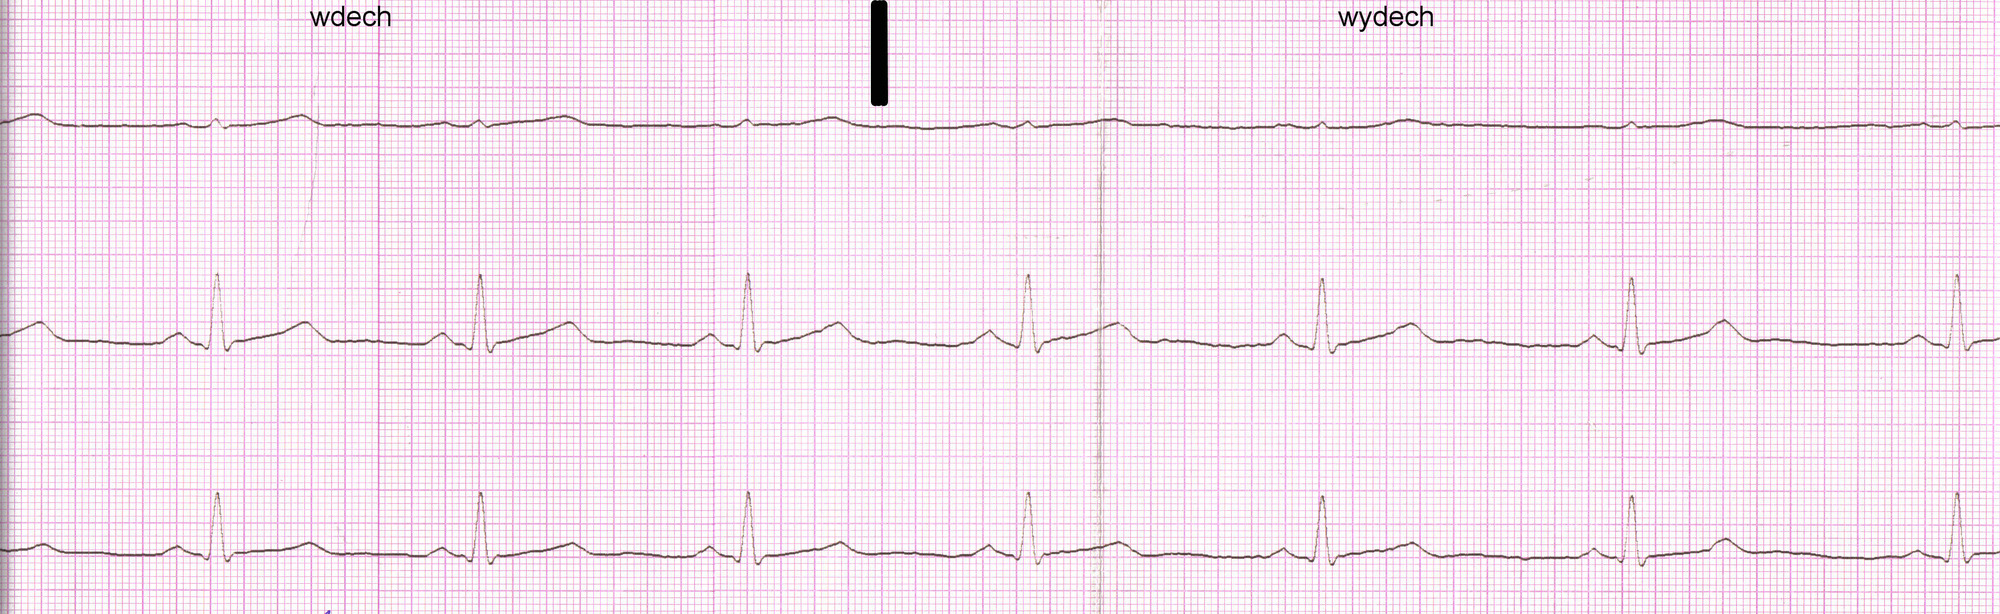
\includegraphics[width=1\linewidth]{EKG_wykres.jpg}
    \caption{\cite{2} Elektrokardiogram zdrowego, 21-letniego mężczyzny. Zaznaczony wdech i wydech.}
    \label{fig:ekg}
\end{figure}

\section{Anomalie występujące w sygnałach EKG}
Anomalie są wszędzie...

\section{Zbiór danych wybrany do projektu}
Ach te dane...

\section{Algorytmy użyte w projekcie}
Alg Alg Algorytmy...

\section{Biblioteka Heartpy}
Opis biblioteki...

\section{Filtrowanie szumu z sygnału}
Ach te filtry...

\section{Cechy uzyskane z Heartpy}
\begin{itemize}
    \item BPM — uderzenia serca na minutę \textit{(eng. Beats per minute)}, tętno; obliczane jako średni odstęp między uderzeniami serca w całym analizowanym sygnale (segmencie)
    \item IBI — odstęp między kolejnymi uderzeniami serca
    \item SDNN — odchylenie standardowe odstępów RR
    \item SDSD — odchylenie standardowe kolejnych różnic
    \item RMSSD — średnia kwadratowa kolejnych różnic
    \item PNN20 — odsetek kolejnych różnic powyżej 20 ms
    \item PNN50 — odsetek kolejnych różnic powyżej 50 ms
    \item HR\_MAD — medianowe odchylenie bezwzględne odstępów RR
    \item SD1 — odchylenie standardowe prostopadłe do linii identyczności (parametry Poincaré)
    \item SD2 — odchylenie standardowe wzdłuż linii identyczności
    \item S — pole elipsy opisanej przez SD1 i SD2
    \item SD1/SD2 - stosunek SD1 do SD2
    \item BREATHING RATE — to częstotliwość oddechu, z którą bicie serca jest silnie związane
\end{itemize}

\section{Typowe podejścia do problemu}
\cite{3} Można wytrenować wiele różnych rodzajów algorytmów uczenia maszynowego w celu wykrywania anomalii. Do najpopularniejszych metod wykrywania anomalii należą:

\subsection{Algorytmy oparte na gęstości}
Algorytmy oparte na gęstości określają, kiedy wartość odstająca różni się od większego, a zatem gęstszego normalnego zestawu danych, przy użyciu algorytmów takich jak K-najbliższy sąsiad i las izolacyjny.

\subsection{Algorytmy oparte na klastrach}
Algorytmy oparte na klastrach oceniają, w jaki sposób dowolny punkt różni się od skupień powiązanych danych, przy użyciu technik takich jak analiza skupień K-średnich.

\subsection{Algorytmy sieci Bayesa}
Algorytmy sieci Bayesa opracowują modele służące do szacowania prawdopodobieństwa wystąpienia zdarzeń na podstawie powiązanych danych, a następnie identyfikowania znaczących odchyleń od tych przewidywań.

\subsection{Algorytmy sieci neuronowych}
Algorytmy sieci neuronowych uczą sieć neuronową przewidywania oczekiwanych szeregów czasowych, a następnie oznaczania odchyleń.

\section{Wnioski}
Wszyscy kochamy wnioski...

\newpage
\bibliographystyle{alpha}
\bibliography{bibliography}

\end{document}
